% You should title the file with a .tex extension (hw1.tex, for example)
\documentclass[11pt]{article}

\usepackage{hyperref}
\hypersetup{
    colorlinks=true,
    linkcolor=blue,
    filecolor=blue,      
    urlcolor=blue,
    citecolor=black,
}
\usepackage{amsmath}
\usepackage{mathtools}
\usepackage{amssymb}


\oddsidemargin0cm
\topmargin-2cm     %I recommend adding these three lines to increase the 
\textwidth16.5cm   %amount of usable space on the page (and save trees)
\textheight23.5cm  

\setlength{\parindent}{0pt}
\setlength{\parskip}{5pt plus 1pt}
 
\DeclarePairedDelimiter\abs{\lvert}{\rvert}

\begin{document}

\medskip                        % Skip a "medium" amount of space
                                % (latex determines what medium is)
                                % Also try: \bigskip, \littleskip


\thispagestyle{plain}
\begin{center}                  % Center the following lines
{\Large EPI scaling} \\
Sean Bittner \\
September 17, 2020 \\
\end{center}

\section{Introduction}
A relative strength of EPI is its scalability in parameter dimension $|z|$. 
This write-up compares the performance of EPI to SMC-ABC and SNPE as $|z|$ is increased.  
The application is to condition arbitrary rank-2 RNNs on a regime of stable amplification.

\textbf{SMC-ABC}: 
Traditional approaches to likelihood-free inference -- approximate Bayesian computation (ABC) methods -- randomly sample parameters $z$ until a suitable set is obtained.
State-of-the-art ABC methods leverage sequential monte-carlo (SMC) sampling techniques to obtain parameter sets more efficiently.
To obtain more parameter samples, SMC-ABC must be run from scratch again.
ABC methods do not confer log probabilities of samples.

\textbf{SNPE}: Like EPI, sequential neural posterior estimation (SNPE) uses deep learning to produce flexible posterior approximations.
Like traditional Bayesian inference methods, SNPE conditions directly on the statistics of data.
This differs from EPI, where posteriors are conditioned on emergent properties (moment constraints on the posterior predictive distribution).
Peculiarities of SNPE (density estimation approach, two deep networks) make scaling in $z$ prohibitive.

\textbf{Rank-2 RNN}: The model we use is a rank-2 RNN with N neurons:
\begin{equation*}
U = \begin{bmatrix} u_1 & u_2 \end{bmatrix}, V = \begin{bmatrix} v_1 & v_2 \end{bmatrix}, J = UV^\top, \text{\hspace{2cm}}
u_1, u_2, v_1, v_2 \in \left[-1, 1 \right]^N
\end{equation*}
\begin{equation*}
\tau \dot{r} = -r + Jr
\end{equation*}
From \cite{bondanelli2020coding}, we know necessary and sufficient conditions for RNNs to exhibit stable amplification.  These two conditions are on the maximal real eigenvalue of $J$ ($\text{real}(\lambda_1)$) and the maximal eigenvalue of $J^s = \frac{J + J\top}{2} (\lambda^s_1)$:
\[\text{real}(\lambda_1) < 1, \lambda^s_1 > 1\]

In our analysis, we seek to condition rank-2 networks of increasing size on a regime of stable amplification.  
Networks with $\text{real}(\lambda_1) = 0.5 \pm 0.5$ and $\lambda_1^s = 1.5 \pm 0.5$ will yield moderate (quantifiable) amplification.

\underline{EPI emergent property}: EPI can naturally condition on this emergent property.
\[\mathbb{E}\begin{bmatrix} \text{real}(\lambda_1) \\ \lambda^s_1 \\ (\text{real}(\lambda_1)-0.5)^2 \\ (\lambda^s_1 -1.5)^2  \end{bmatrix} = \begin{bmatrix} 0.5 \\ 1.5 \\ 0.25^2 \\ 0.25^2 \end{bmatrix}\]

\underline{SNPE observation}: SNPE cannot condition on the variance of observations across posterior.  Thus, we condition on an observation $x_0$ located at the mean of our desired emergent property.
\[x_0 = \begin{bmatrix} \text{real}(\lambda_1) \\ \lambda^s_1 \end{bmatrix} = \begin{bmatrix} 0.5 \\ 1.5 \end{bmatrix} \]

\underline{SMC-ABC criteria}: ABC methods define tolerance $\epsilon$ and distance for observed data $x_0$.\\
\begin{center}
$\epsilon = 0.5$, $l2$ distance, and  $x_0 = \begin{bmatrix} \text{real}(\lambda_1) \\ \lambda^s_1 \end{bmatrix} = \begin{bmatrix} 0.5 \\ 1.5 \end{bmatrix}$
\end{center}

\clearpage

\section{Results}
SMC-ABC was run with \href{https://pyabc.readthedocs.io/en/latest/index.html}{pyabc} package.  SNPE was run with \href{http://www.mackelab.org/delfi/}{delfi} package.  EPI was run with revision branch of \href{https://github.com/cunningham-lab/epi/tree/revision}{epi} package.  All methods use a uniform prior form -1 to 1 for each parameter.

\begin{figure}[h]
\begin{center}
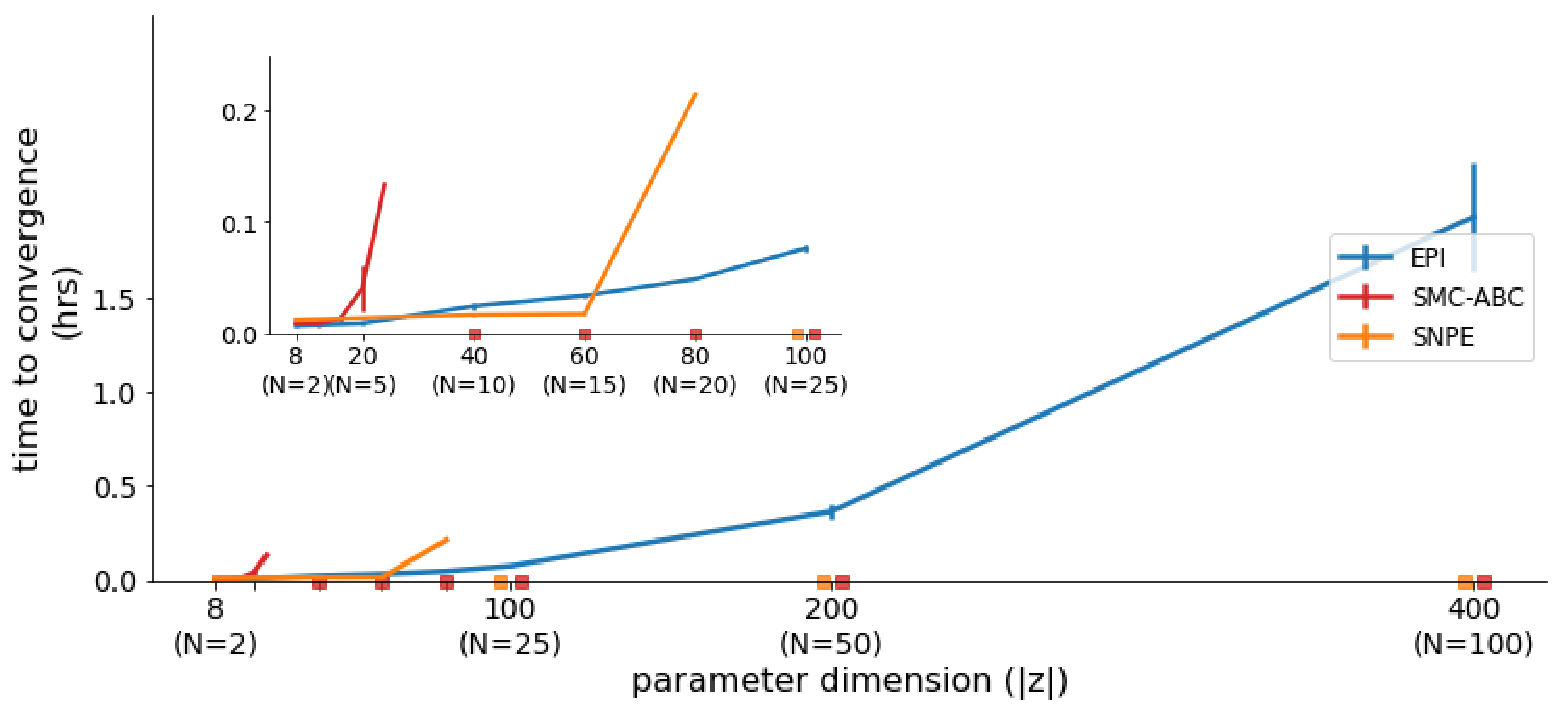
\includegraphics[scale=.4]{epi_both.png} \\
\end{center}
\caption{\small EPI scales with $z$ to high dimensions. 
Square - algorithm never converged across all experiments.
Convergence definitions: 
EPI (blue) - satisfies all moment constraints, 
SNPE (orange)- produces at least 1/10,000 parameter samples in the bounds of emergent property (mean +- 0.5), 
and SMC-ABC (red) - 100 particles with $\epsilon < 0.5$ are produced.}
\end{figure}

\begin{figure}[h]
\begin{center}
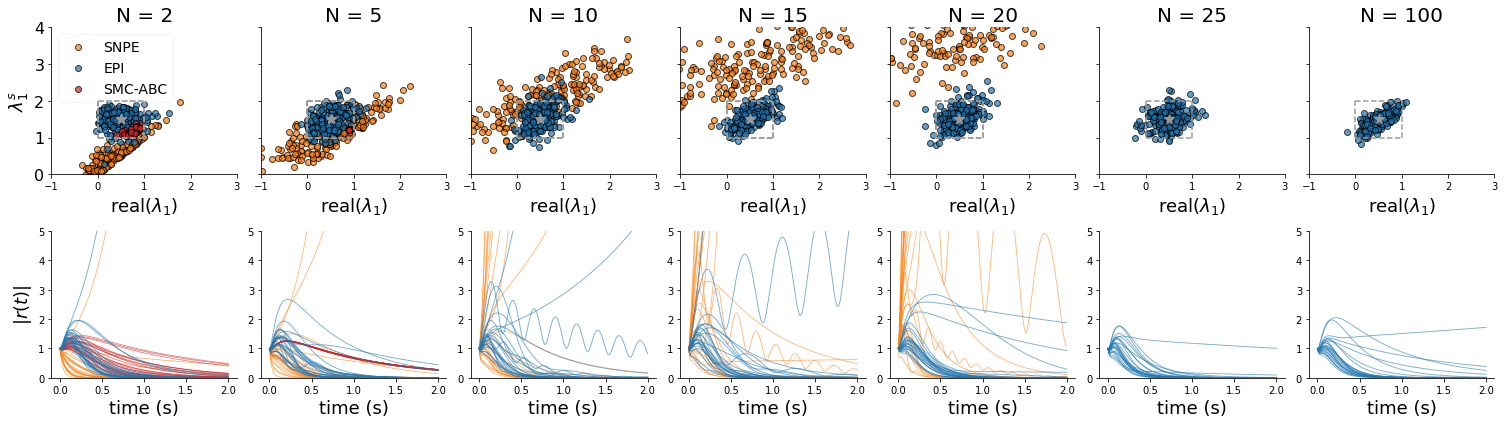
\includegraphics[scale=.3]{EPI_scaling3.png}
\caption{\small Emergent property fidelity.  Top row: Posterior predictive distributions of EPI (blue), SNPE (orange), and SMC-ABC (red). 
Gray star indicates emergent property mean, and gray dashed lines indicate two standard deviations corresponding to the variance constraint.
For $N <= 6$ where SMC-ABC converges, samples are not diverse (path degeneracies).  
For $N >= 25$, SNPE does not produce a posterior approximation yielding parameters with simulations near $x_0$. 
Bottom row: simulations of network parameters resulting from each method ($\tau=100ms$).  Each trace corresponds to simulation of one $z$.  
Almost all EPI networks, few SNPE networks, and all SMC-ABC networks exhibit stable amplification.  
There is little variation in SMC-ABC network simulations.}
\end{center}
\end{figure}

\bibliography{epi_scaling}
\bibliographystyle{unsrt}
\end{document}

